\section{Yolo You Only Look Once}

\begin{figure}
  \centering
  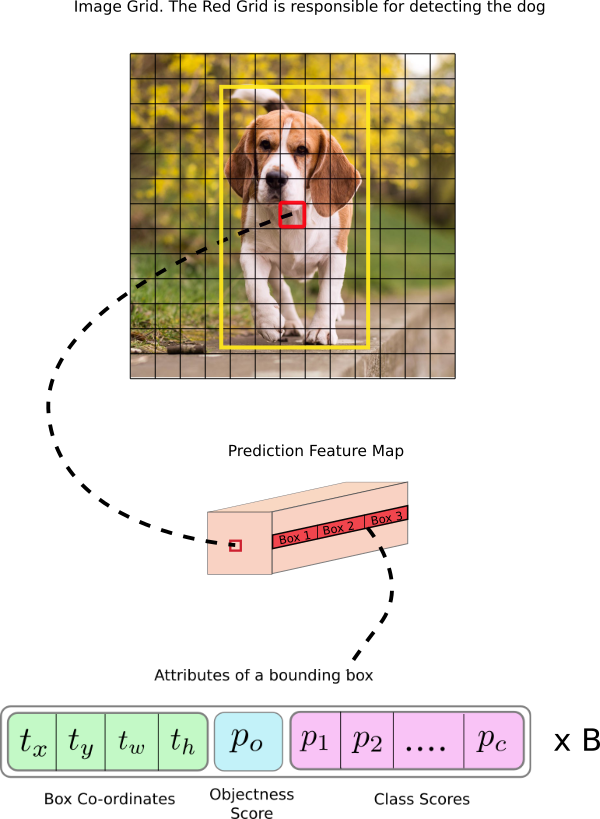
\includegraphics[width=0.8\textwidth]{images/yolo/grid.png}
  \caption{Image Grid}
\end{figure}

Yolo1 splits the image in a 7x7 grid. Each cell predicts a bounding box.\\

In Yolo2 different scales to recognize smaller objects are used. Predicts anchor boxes instead of bounding boxes. The idea is, it is easier to predict the offset of predefined bounding boxes than to classify the bounding box itself. Uses Darknet-19 (Fig \ref{fig:darknet}) and BatchNormalization.

\begin{figure}[H]
  \centering
  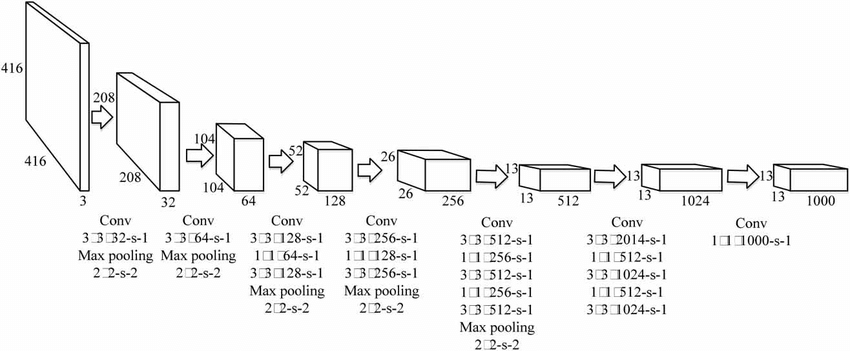
\includegraphics[width=0.5\textwidth]{images/yolo/darknet.png}
  \caption{DarkNet}
  \label{fig:darknet}
\end{figure}

Yolo3 changes to Darknet-53 and uses three scales by using three different sizes of anchor boxes.\\

Yolo4 has been developed by Chien-Yao Wang, developer of CSPBlock. It uses the mish action function and calculates the CIOU, complete intersection over union. It uses CSPDarknet53 (Head) + Spatial Pyramid Pooling + PANet(Neck)\\

Yolo5 is anchorfree. \\

Yolo7 has been developed again by Chien-Yao Wang. \\

Yolo8 uses self attention.\\

Yolo9 is based on Yolo7. It introduces Programmable Gradient Information and improves the backbone using Generalized Efficient Layer Aggregation Network (GELAN).
YoloE \textgreater{} YoloC \textgreater{} (YoloM \textgreater{} YoloS
It can perform classification, instance segmentation and panoptic segmentation.
It has three branches: main Branch, auxiliary branch and multi-evel auxiliary branch which combines gradients from different prediction heads to consider all object sizes
Non-maximum-suppression is used to remove duplicate predictions.

\subsection{Sources}
\begin{enumerate}
  \item \href{https://blog.paperspace.com/how-to-implement-a-yolo-object-detector-in-pytorch/}{How to implemenet Yolo}
  \item \href{https://www.superannotate.com/blog/yolo-object-detection}{Yolo Object Detection}
  \item \href{https://arxiv.org/pdf/1911.11929.pdf}{CASPNet-Backbone}
\end{enumerate}